% Created 2020-10-06 mar 18:24
% Intended LaTeX compiler: pdflatex
\documentclass[presentation,aspectratio=169, usenames, dvipsnames]{beamer}
\usepackage[utf8]{inputenc}
\usepackage[T1]{fontenc}
\usepackage{graphicx}
\usepackage{grffile}
\usepackage{longtable}
\usepackage{wrapfig}
\usepackage{rotating}
\usepackage[normalem]{ulem}
\usepackage{amsmath}
\usepackage{textcomp}
\usepackage{amssymb}
\usepackage{capt-of}
\usepackage{hyperref}
\usepackage{khpreamble}
\usepackage{amssymb}
\usepgfplotslibrary{groupplots}
\usepackage{pgfplotstable}
\newcommand*{\shift}{\operatorname{q}}
\definecolor{ppc}{rgb}{0.1,0.1,0.6}
\definecolor{iic}{rgb}{0.6,0.1,0.1}
\definecolor{ddc}{rgb}{0.1,0.6,0.1}
\usetheme{default}
\author{Kjartan Halvorsen}
\date{2020-10-06}
\title{Process Automation Laboratory  - Anti-windup assignment}
\hypersetup{
 pdfauthor={Kjartan Halvorsen},
 pdftitle={Process Automation Laboratory  - Anti-windup assignment},
 pdfkeywords={},
 pdfsubject={},
 pdfcreator={Emacs 26.3 (Org mode 9.3.6)}, 
 pdflang={English}}
\begin{document}

\maketitle


\section{Context}
\label{sec:org7348bef}
\begin{frame}[label={sec:orgccface9}]{The two-tank system}
\begin{center}
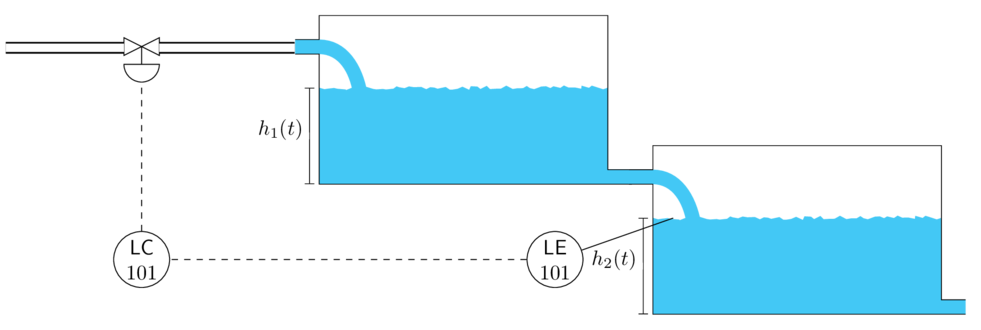
\includegraphics[width=0.8\linewidth]{../../figures/two-tanks-shutoff-valve.png}
\end{center}
\end{frame}


\section{Anti-windup}
\label{sec:orge5ed4e3}

\begin{frame}[label={sec:org755088d}]{Anti-windup using back-calculation - Spot the mistake}
\begin{center}
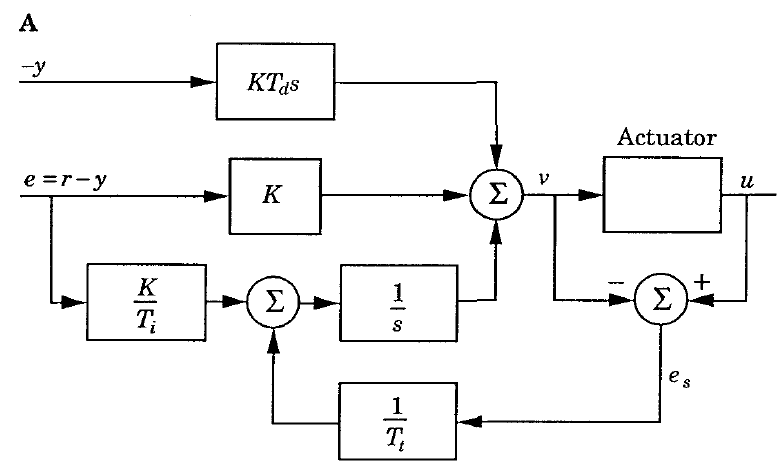
\includegraphics[height=0.38\textheight]{../../figures/astrom-back-tracking.png}
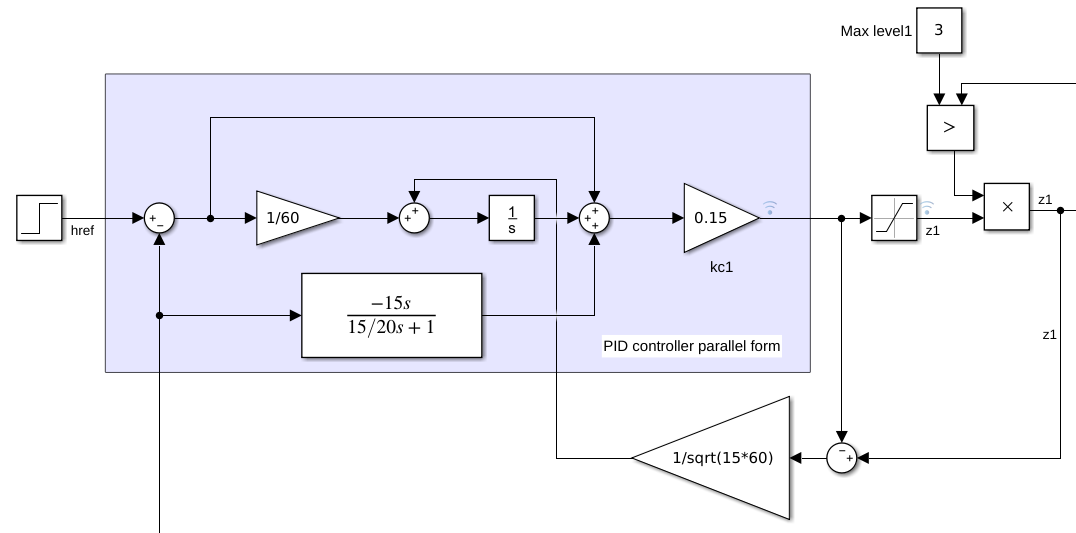
\includegraphics[height=0.42\textheight]{../../figures/back-tracking-review.png}
\end{center}
\end{frame}


\begin{frame}[label={sec:orgede0024}]{Anti-windup using back-calculation}
\begin{center}
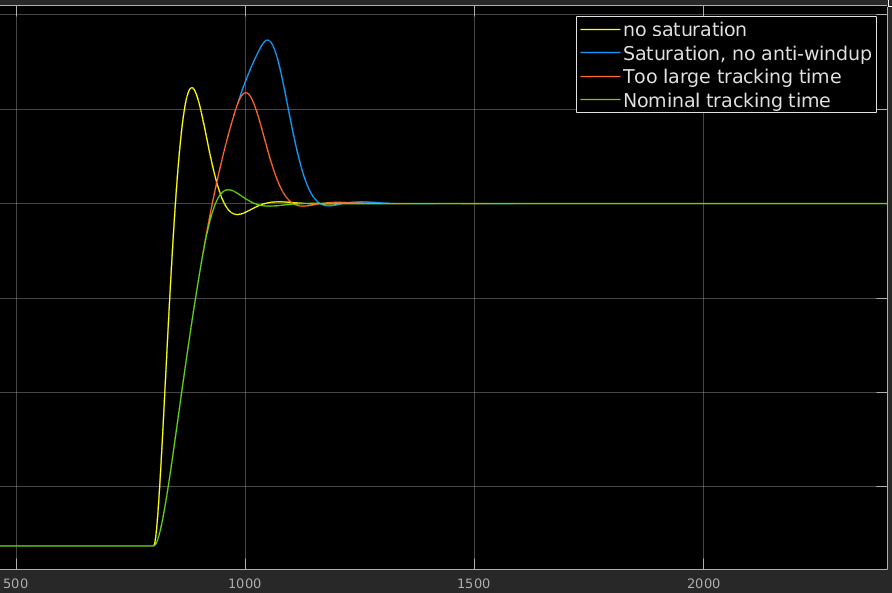
\includegraphics[width=.82\linewidth]{../../figures/antiwindup-review.png}
\end{center}
\end{frame}
\end{document}